\chapter{Použité webové technológie}
\label{kapitola3}
V tejto kapitole sa čitateľ oboznámi s použitými webovými technológiami v aplikácie. Na úvod sa uvádza popis zvolenej databáze

\section{Databáza}
V tejto sekcii sa čitateľ zoznámi s NoSQL databázou MongoDB a knižnicou Mongoose.

\subsection{MongoDB}
\label{mongodb}
MongoDB\cite{mongodb} je open-source nerelačná databáza založená na dokumentoch. Namiesto používania tradičných tabuliek a riadkov relačnej databáze, MongoDB vytvára kolekcie ktoré sa skladajú z dokumentov vo formáte JSON. Jednotlivé dokumenty sa skladajú z párov kľúč-hodnota. Každý dokument môže mať rozlišný počet položiek. Veľkosť a obsah jednotlivých dokumentov sa môže taktiež od seba líšiť. Štruktúra dokumentu sa viac podobá štruktúre, ktorú vývojári vytvárajú pri programovaní tried a objektov. 

\subsection{Mongoose.js}
\label{mongoose}
Mongoose.js je Node.js knižnica pre dátové modelovanie objektov pre MongoDB. Uľahčuje užívateľom prácu s MongoDB prekladaním dokumentov z databáze na objekty. Spravuje vzťahy medzi dátami, poskytuje validáciu schémy, typovanie a používa sa pre modelovanie dátových modelov na MongoDB objekty. Poskytuje dopytovacie funkcie nad modelmi, pomocou ktorých sa získavajú a ukladajú dáta do databáze. Tieto funkcie sú reťazovatelné(chainable). 

Mongoose používa schémy pre modelovanie a správu dát v MongoDB. Schéma popisuje atribúty jednotlivých položiek s ktorými aplikácia pracuje, napríklad jeho dátový typ, či je položka povinná, alebo voliteľná. 

\section{TypeScript}
\label{typescript}
Aby sa porozumela logika a nápad za vytvorením TypeScriptu a použitím ho v tomto projektu, je nutné sa najprv zoznámiť s nevýhodami JavaScriptu. JavaScript\cite{typescript} umožní zo statického webu vytvoriť dynamické aplikácie, ktoré používame dodnes. Písať zdrojový kód čisto v JavaScriptu je pomerne náročné a pri väčších projektoch takmer nemožné. Samotný jazyk neumožňuje počas programovania uvádzať dátové typy, čo veľmi sťažuje nápovedu v kóde a tiež jeho automatickú kontrolu.

TypeScript\cite{typescript} bol vytvorený v roku 2012 firmou Microsoft a jeho zdrojový kód je dostupný pre verejnosť. Jedná sa o nadstavbu jazyka JavaScript. Rozširuje ho o triedy, rozhrania, statické typovanie a ďalšie funkcionality z objektovo orientovaného programovania. TypeScript je využívaný aj spoločnosťou Googlu, ktorá ho integrovala do JavasSriptového frameworku Angular.

Ako už bolo spomenuté, TypeScript umožňuje programátorom statické typovanie. Existujú dva základné typové systémy:
    \begin{itemize}
        \item Pri \textbf{dynamickom typovaní} premenná má nastavený dátový typ, ale systém typ skrýva a nedáva ho vôbec najavo. Premenné pri dynamickom typovaní mnohokrát ani nemusia byť deklarované, akonáhle sa do nejakej premennej niečo uloží a jazyk zistí, že nebola nikdy deklarovaná, sám ju založí. Do tej istej premennej sa môže ukladať reťazec, potom objekt a potom pole. Jazyky využívajúce dynamický typovanie vnútorne automaticky menia dátový typ. V týchto jazykoch je vývoj rýchlejší vďaka menšiemu množstvu kódu, zástupcovia sú napríklad Python, alebo práve JavaScript.
        \item Pri \textbf{statickom typovaní} je striktne vyžadované definovanie typu premennej a typ je naďalej nemenný. Pri uložení hodnoty iného typu do premennej, kompilácia zdrojového kódu skončí chybovím hlásením.
    \end{itemize}
    
    TypeScript\cite{typescript} je typizovaním jazykom, všetky premenné musia byť najprv deklarované s priradeným dátovým typom. Nevýhodou je, že vďaka deklaráciám je zdrojový kód objemnejší a vývoj pomalší. Naopak obrovskou výhodou je, že kompilátor pred spustením skontroluje, či všetky nastavené hodnoty vyhovujú ich dátovým typom. Dynamické typovanie síce vyzerá ako výhodné, ale pri čítaní zdrojového kódu je ťažké zistiť typ hodnoty premennej. TypeScript do základnej mieri tiež povoľuje využitie dynamických typov cez takzvané \texttt{union typy}. Union typy umožňujú nastavenie viacero dátových typov premennej, napríklad \texttt{let data: string | number}, kde premenná \texttt{data} môže obsahovať reťazec, alebo číslo. TypeScript pri priradení hodnoty nesprávneho dátového typu nedovolí program ani skompilovať a na chybu ihneď upozorní.
\section{Frontend}
TODO

\subsection{HTML}
Hypertextový značkovací jazyk\cite{html}, alebo skrátene HTML je jazyk vytvorený Timom Berners-Leeom v roku 1991. Hneď na začiatku treba zdôrazniť, že sa nejedná o programovací jazyk. HTML neumožňuje vytváranie premenných, alebo funkcií. Jazyk je určený na vytváranie webových stránok a na organizovanie, formátovanie rôznych informácií zobraziteľných vo webovom prehliadači. Umožňuje užívateľom vytvárať 
a štrukturovať sekcie, nadpisy, paragrafy, odkazy a mnoho ďalších pre webové stránky a aplikácie. Pri práci s HTML sa používajú štruktúry, ktoré sa nazývajú \texttt{značky(tagy)} a \texttt{atribúty}, pomocou ktorých sa štrukturujú jednotlivé časti web stránky. 

\subsection{CSS}
Kaskádové štýly\cite{css}, alebo skrátene CSS je rozšírenie jazyka HTML. Jazyk bol vytvorený a je udržiavaný skupinou v organizácii W3C\footnote{Skupina ľudí, ktorá navrhuje vylepšenia a špecifikácie o Internete a jeho vývoji.}.  Prvá verzia vznikla v roku 1996 a obsahovala iba modifikácie písmen, okrajov a farieb. Súčasná verzia je \texttt{CSS3}. Jazyk umožňuje vizuálne formátovanie internetových dokumentov a špecifikuje ako sa majú dokumenty prezentovať pre užívateľa. Pomáha v štýlovaní jednotlivých elementov a v upravovaní ich umiestnenia. Využíva sa od základných 
štýlov, ako zmena farby textu, alebo veľkosti až k rozsiahlejším zmenám rozloženia, a aj pre zobrazovanie animovaných efektov. 

V súčasnej dobe sa často používajú preprocesory pri práci s CSS. V aplikácii sa využíva preprocesor \texttt{Sass}. Preprocesor\cite{sass} je program ktorého, výstup je spracovaný ďalším programom, t.j. štýly napísané v Sass sú spracované ďalším programom z čoho vznikne CSS. Hlavným dôvodom ich použitia je prehľadnosť kódu a súborov. Medzi najpopulárnejšie preprocesory patrí Sass, Less a Stylus.

\subsection*{Sass}
\label{sass}
Sass\cite{sass} je najstarším CSS preprocesorom. Je ľahko naučiteľný a pomerne jednoduchý jazyk. Medzi jeho hlavné výhody patrí vytváranie premenných a uchovávanie hodnôt do nich, vytváranie vnorených štýlov, matematických operácií, cyklov a funkcií. Sass naďalej podporuje importovanie externých súborov, čo umožňuje rozdelenie štýlov do rôznych logických častí. Jednotlivé celky sa potom preprocesorom skompilujú do jedného CSS súboru. 

\subsection*{Buefy}
\label{buefy}
Buefy poskytuje predpripravené komponenty pre užívateľské rozhranie. Uľahčuje prácu vývojárom so štýlovaním základných elementov dokumentu. V aplikácii sa využíva komponenta pre tlačítka, skrývanie obsahu, dialógy, kolónky vstupu užívateľa, vykreslovanie ikón, animáciu načítania, navigačný panel a bočný panel. Zdrojový kód frameworku je voľne dostupný pre verejnosť. Každá komponenta je responzívna, sama sa prispôsobuje rôznym rozlíšeniam obrazovky a týmto uľahčuje vývoj aj pre mobilnú platformu. 

Framework je vytvorený vo Vue.js a zakladá sa na CSS knižnici Bulma. Bulma je taktiež open-source knižnica, ktorá je postavená na CSS architektúre \texttt{flexbox}. Samotná knižnica poskytuje CSS triedy pre štýlovanie HTML dokumentu. Buefy pomocou týchto tried vytvorí jednotlivé komponenty užívateľského rozhrania pre Vue.js, ktoré sú potom jednoducho použiteľné v aplikácii. Tieto komponenty sa označujú predponou \texttt{b-}, napríklad \texttt{<b-button></b-button>}.

\subsection{Vue.js}
\label{vue}
Vue.js\cite{vue-guide} patrí medzi najpopulárnejšie nástroje pre tvorbu jednostránkových aplikácii. Je výkonný, rýchly a minimalistický. Veľkou výhodou je, že patrí medzi progresívne frameworky, t.j. našu aplikáciu vieme rozdeliť na viacero častí, ktoré môžu byť samostatne vyvíjané. Stal sa jedným z obľúbených kvôli jeho jednoduchosti. Má veľmi prehľadnú a pestrú dokumentáciu v anglickom aj čínskom jazyku.

Framework bol vytvorený Evanom Youom, ktorý pracoval v Googlu a Meteoru. V Googlu začal používať AngularJS, ktorým sa inšpiroval, ale tento framework mu nevyhovoval kvôli jeho striktnému písaniu kódu. Jeho motiváciou bolo vziať najlepšie vlastnosti Angularu a vytvoriť z nich nástroj, ktorý mu zjednoduší a zefektívni prácu.

Dizajn Vue.js sa inšpiroval MVVM\footnote{Model-View-ViewModel} architektúrou. Zameriava sa na vrstvu pohľadu. Spája pohľad a model cez dvojstrannú väzbu (anglicky two-way binding), ako je vidieť na obrázku \ref{pic:mvvm}. Ostatné funkcionality SPA, ako smerovanie a úložisko(ďalej označované aj ako store) môžu byť doplnené cez pomocné knižnice.
    \begin{figure}[!hbt]
        \centering
        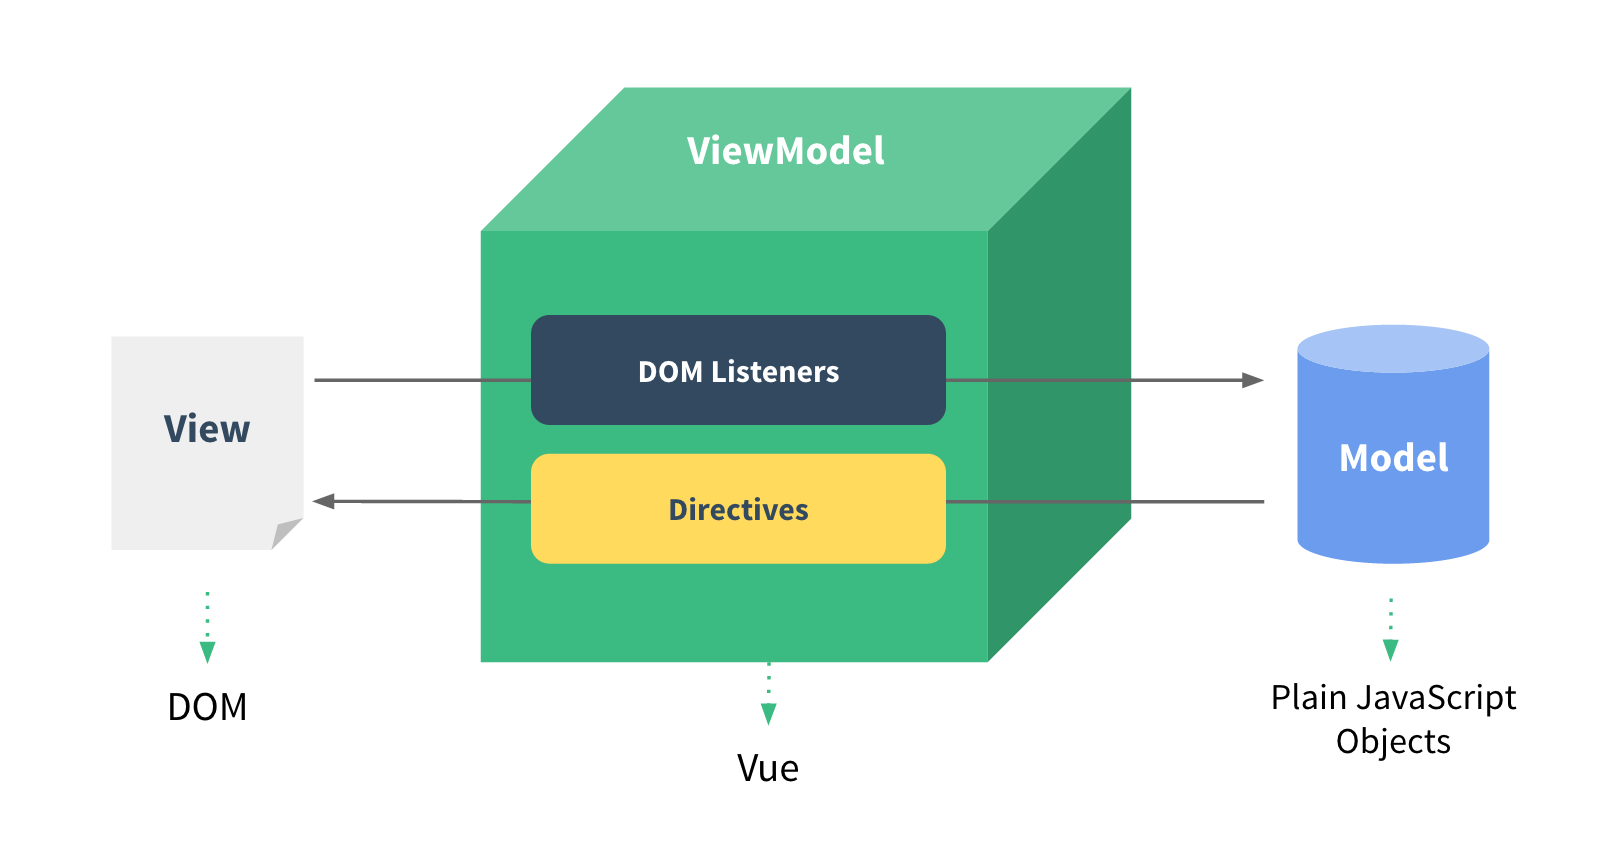
\includegraphics[scale=0.2]{obrazky/mvvm.png}
        \caption{Znázornenie úlohy Vue.js v MVVM architektúre \cite{vue-guide}.}
        \label{pic:mvvm}
    \end{figure}

\subsection*{Inštalácia}
Vue.js bol vytvorený aby bol ľahko osvojiteľný a a použiteľný. Môže byť začlenený do projektu viacerými spôsobmi. 

Štyri hlavné spôsoby sú nasledovné:
    \begin{itemize}
        \item Importovanie balíčka do HTML stránky cez CDN:
        \begin{verbatim}<script src="https://unpkg.com/vue@next"></script>\end{verbatim}
        \item Stiahnutie JavaScriptových súborov a importovanie ich rovnakým spôsobom ako u CDN
        \item Inštalácia cez správcu balíčkov npm
        \item Použitie oficiálneho CLI pre zkonštruovanie projektu
    \end{itemize}
    
\subsection*{Komponenty}
Komponenty hrajú vo Vue.js veľmi dôležitú rolu, umožňujú tvorbu vysoko škálovateľnej aplikácie, ktorá je poskladaná z malých a znovupoužiteľných častí. Môžeme mať komponenty napríklad pre hlavičku, bočný panel, obsah, ktoré môžu obsahovať ďalšie komponenty pre zoznam prezentácií, výpis detailu prezentácie. Výsledkom rozdelenia do jednotlivých častí je ľahko udržateľný a prehľadný zdrojový kód. Komponenty tvarujú hierarchiu vnoreného stromu, ktorý je znázornený na obrázku \ref{pic:components}. Tento strom reprezentuje aplikačné rozhranie.
    \begin{figure}[!hbt]
        \centering
        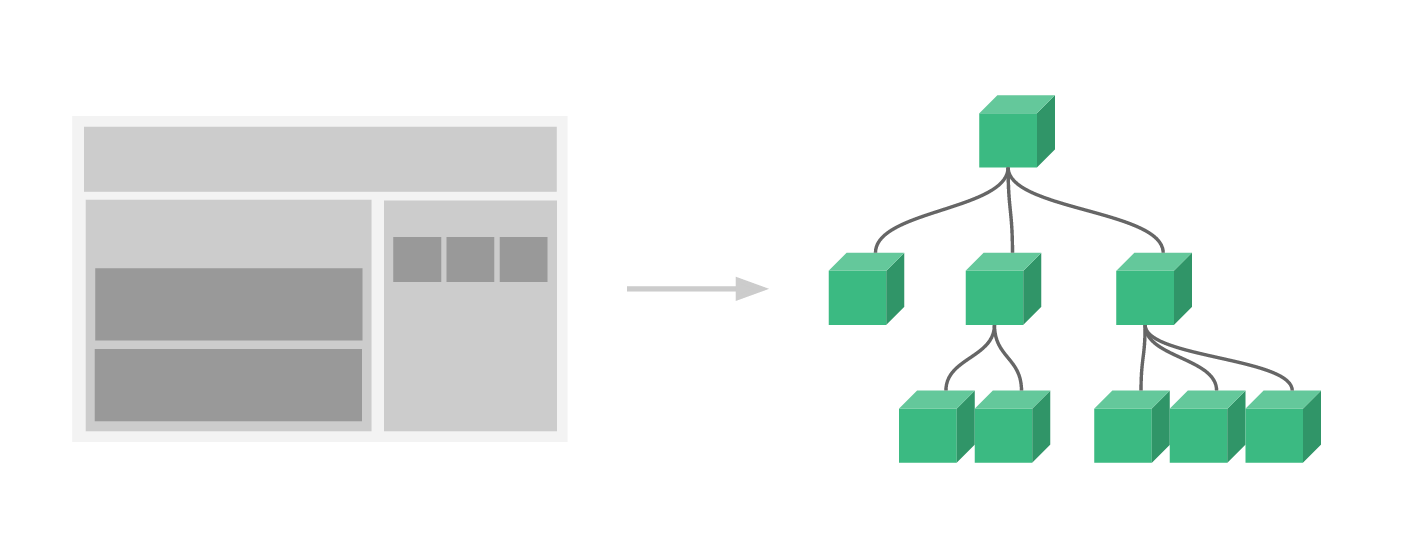
\includegraphics[scale=0.25]{obrazky/components.png}
        \caption{Znázornenie komponentov ako vnorený strom\cite{vue-guide}.}
        \label{pic:components}
    \end{figure}
    
\subsection*{Registrovanie komponentov}
Existujú dva postupy registrovania jednotlivých komponentov: \textit{lokálne} a \textit{globálne}. Lokálne komponenty je potrebné pred každým použitím importovať, narozdiel od globálnych, ktoré stačí zaregistrovať raz a môžu byť použité v šablóne hociktorej komponenty. 

Typický príklad pre globálnu komponentu je dizajnový prvok, ako napríklad animácia pri načítaní údajov, označovaný ako spinner. Tento typ animácie sa používa pri každom načítaní údajov, na viacerých miestach v aplikácii. Aby sme ho nemuseli po každom importovať stačí keď si ho raz globálne zaregistrujeme a môžme ho voľne používať. 

Príklad lokálnej komponenty je formulár pre registrovanie užívateľa, ktorý sa pravdepodobne použije iba raz a nepotrebujeme mať k nemu prístup v celej aplikácii.

\subsection*{Komunikácia medzi komponentami}
Komponenty začnú byť ešte viac užitočné pri vymieňaní údajov medzi sebou. Štandardne, každá jedna komponenta je izolovaná, čo znamená, že nemá prístup k rodičovským údajom. Majme komponentu pre stručný výpis informácií o prezentácii, po kliknutí na ňu sa zobrazí ďalšia komponenta s detailným výpisom. Pri tomto príklade potrebujeme predať informácie o prezentácii z jednej komponenty na druhú. Na komunikáciu medzi rodičom a potomkom sa používa \texttt{props} a metóda \texttt{\$emit}.

Props sú atribúty, ktorým vieme nastaviť hodnoty. Slúžia na predanie údajov z rodiča na potomka. Po nadobudnutí hodnoty sa z nich stanú premenné použiteľné v komponente. Počet props nie je obmedzený a prijíma ľubovolný typ údajov.

Metóda \$emit slúži na komunikáciu opačným smerom. Pomocou tejto metódy vieme vytvoriť vlastnú udalosť, ktorú rodič môže odpočúvať. Majme komponentu potomka v ktorej sa nachádza tlačítko. Kliknutím na tlačítko sa zavolá metóda \$emit do ktorej sa predá meno udalosti a voliteľné dáta. Rodičovská komponenta môže odchytiť túto udalosť a reagovať na ňu. Vysielanie udalostí je užitočné keď máme viacero potomkov s rovnakou logikou, týmto spôsobom nemusia všetky tieto komponenty obsahovať tú istú logiku, stačí keď bude implementovaná iba v rodičovskej komponente a pristúpi sa k nej cez \$emit.

\subsection*{Životný cyklus komponenty}
Vo Vue.js každá komponenta je samostatná Vue inštancia\footnote{Jeden konkrétny exemplár triedy} a každá inštancia má svoj životný cyklus. Životný cyklus komponenty sa skladá z niekoľkých krokov, ako napríklad jej vytvorenie, pripevnenie inštancie k DOM\footnote{Objektový model HTML dokumentu}, aktualizácia DOM-u pri zmene údajov alebo jej zrušenie. Vývojári majú pri každom kroku možnosť pridania vlastného kódu cez \texttt{funkcie životného cyklu (lifecycle hooks)}. Medzi najpoužívanejšie patria:
    \begin{itemize}
        \item\texttt{beforeCreated} - Volá sa hneď po inicializácii inštancie, ktorá zatiaľ nič neobsahuje.
        \item\texttt{created} - Pri tomto kroku sa dokončilo nastavenie pozorovania dát, computed premenných, metód a udalostí. Zatiaľ nemáme prístup k DOM. Môže sa použiť pre registrovanie vlastných udalostí.
        \item\texttt{beforeMount} - Volá sa pred pripevnením DOM.
        \item\texttt{mounted} - Najpoužívanejšia funkcia lifecycle hook. Volá sa po pripevnení inštancie k DOM. V tejto funkcii už máme prístup k jednotlivým elementom v DOM. Častokrát používaná pre sťahovanie dát z API.
        \item\texttt{beforeUpdate} - Volá sa pri zmene dát. Máme prístup k existujúcemu DOM pred jeho aktualizáciou.
        \item\texttt{updated} - Funkcia volaná po znova-vykreslení DOM.
        \item\texttt{beforeUnmount} - Volá sa pred odpojením inštancie od DOM-u.
        \item\texttt{unmounted} - Po tomto kroku je inštancia kompletne odpojená, taktiež jej potomky a udalosti. Používaná pre odpojenie vlastných udalostí.
    \end{itemize}

Pri použití Composition API, o ktorom si povieme viac v sekcii \ref{compositionapi}, sa tieto funkcie trochu líšia. Lifecycle hooky beforeCreated a created sú súčasťou funkcie \texttt{setup()} a pred každý hook treba pridať predponu \texttt{on}: onCreated, onMounted, atď. 

    \begin{figure}[!hbt]
        \centering
        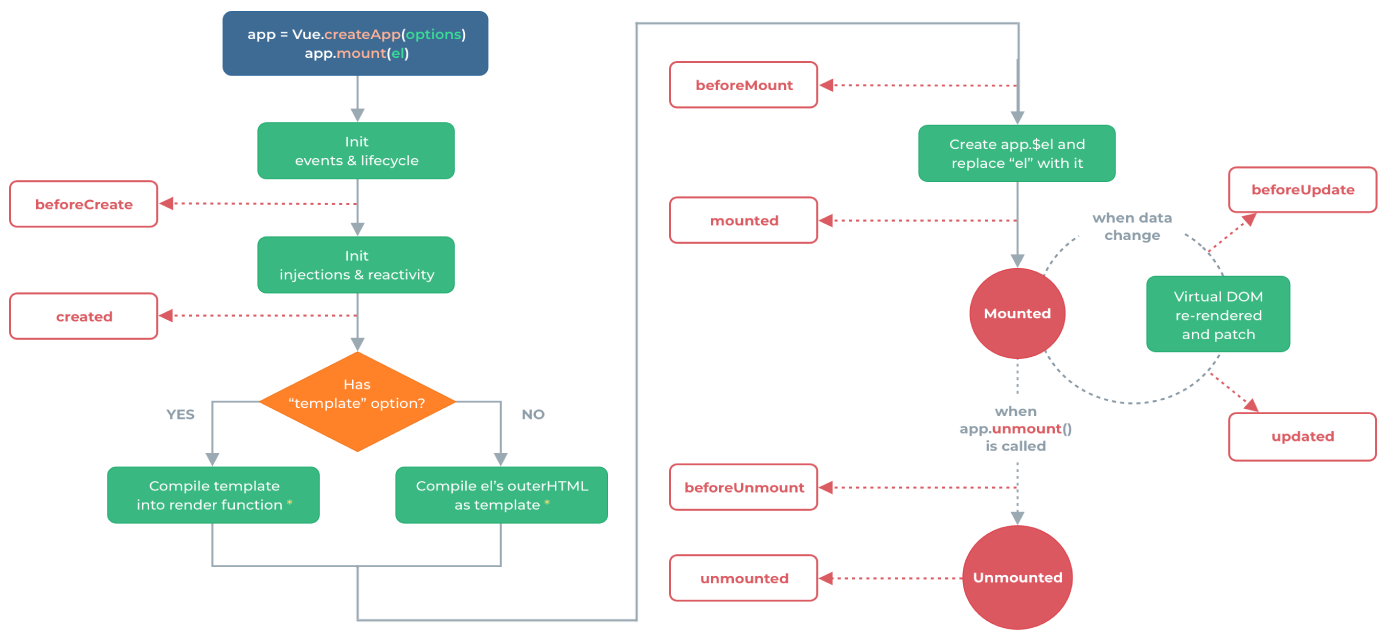
\includegraphics[scale=0.3]{obrazky/lifecycle.png}
        \caption{Graf životného cyklu komponenty\cite{vue-guide}.}
        \label{pic:hooks}
    \end{figure}

\subsection*{Šablóna}
Komponenta sa vykresľuje cez HTML šablónu. Okrem základnej funkcionality jazyka HTML umožňuje aj výpis statických aj dynamických hodnôt, dynamickú aktualizáciu CSS štýlov a tried, použitie podmienok na obmedzenie vykresľovania a použitie cyklov pre prechádzanie hodnôt v poli. V šablóne má vývojár prístup k premenným aj metódam v súbore. Obsah šablóny sa musí nachádzať medzi značkou \texttt{<template>}.

\subsection{Composition API}
\label{compositionapi}
Vue.js verzia 2 priniesla funkcionalitu mixinov. Mixiny boli hlavným nástrojom pre vyčlenenie jednotlivých častí logiky komponenty do znovupoužitelných celkov. Umožňujú tvorbu premenných, funkcií a kódov vo funkciách životného cyklu, rovnakým spôsobom ako v komponentoch. Mixiny avšak spôsobujú viacero konfilktov. Pri ich importovaní sa premenné a funkcie z mixinu zlúčia do súboru komponenty a môžu vzniknúť konflikty rovnakého pomenovania. Ďalším významným problémom je limitovaná znovupoužitelnosť. Mixiny nepodporujú predávanie parametrov pre zmenu logiky, tým pádom majú zredukovanú flexibilitu.

Všetky tieto problémi sa nástupom Composition API vyriešili. Composition API rovnako ponúka vyčlenenie častí logiky a ich znovupoužitie. Avšak neslúži iba pre znovupoužitelnosť, vyčleniť sa môže aj logika, ktorá v komponente zaberá príliš veľa miesta.  Výsledkom je prehľadnejšia komponenta v ktorej sa jednoduchšie orientuje. Súbor, ktorý obsahuje vyčlenenú logiku sa označuje ako \texttt{skladateľný(composable)}. Composition API poskytuje vo vyčlenených súboroch rovnaké funkcionality ako v komponentoch, možnosť deklarovania reaktívnych premenných, computed premenných, funkcií, sledovanie premenných, prístup ku kontextu aplikácie a k funkciám životného cyklu.

Začiatočným bodom v Composition API je funkcia \texttt{setup}. Setup funkcia sa vykoná pred vytvorením komponenty, hneď jak sa atribúty \texttt{props} spracujú. Funkcia prijíma props a kontext aplikácie ako parameter. Všetko čo sa z funkcie vracia je dostupné v komponente a aj v šablóne komponenty. 

\subsection*{Reaktívne premenné}
Composition API umožňuje vytváranie reaktívnych premenných pomocou funkcie \texttt{ref}. Reaktívne premenné slúžia na automatické prekreslenie šablóny pri ich zmene. Príklad zápisu: 
    \begin{verbatim}const currentSlide = ref<number>(1)\end{verbatim}
Ref zoberie danú hodnotu a zabalí ju do \texttt{Proxy} objektu, pomocou ktorej Vue reaguje na zmeny. K samostatnej hodnote objektu sa pristupuje cez atribút \texttt{.value} a cez rovnaký atribút sa taktiež hodnota upravuje. Kvôli tomu sa premenná deklaruje ako konštanta, lebo pri modifikácii sa upravuje hodnota v objektu a nie celý objekt. V šablóne sa k hodnote pristupuje rovno cez objekt a nie je potrebné použiť atribút \texttt{.value}. 

Composition API ponúka taktiež funkciu \texttt{reactive} pre reaktívny zápis premenných. Príklad použitia:
    \begin{verbatim}const presentation = reactive<Presentaion>({
        title: "Moja prezentácia",
        slides: ["Stránka 1", "Stránka 2"]
}) \end{verbatim}
Funkcia zoberie objekt a každú jednu položku priradí do Proxy objektu. Logika za funkciou je pomerne rovnaká ako pri \texttt{ref}, rozdiel je pri prístupe k jednotlivým položkám a ich hodnotám, kde pri \texttt{reactive} nie je potrebné uviesť atribút \texttt{.value}. Pri použití v šablóne je potrebné uviesť objekt aj atribút, napríklad \texttt{presentaton.title}. Tento zápis sa dá zjednodušiť pomocou funkcie \texttt{toRefs}, táto funkcia vyžaduje reaktívny objekt ako parameter a používa sa pri vrátení hodnôt vo funkcii \texttt{setup}. Funkcia \texttt{toRefs} zoberie objekt a vráti každý jeden atribút ako samostatný \texttt{ref} objekt, týmto spôsobom sa k premennej v šablóne pristupuje iba cez atribút, napríklad \texttt{title}. Pomocou \texttt{reactive} vieme jednotlivé premenné ktoré súvisia so sebou zoskupiť do jedného objektu pre prehľadnejšiu orientáciu v zdrojovom kóde. 

Ako je v hore uvedených príkladoch vidieť, obe reaktívne funkcie podporujú typovanie pomocou TypeScriptu. Typ sa uvádza medzi zátvorky \texttt{<} a \texttt{>}.

\subsection{Nuxt.js}
\label{nuxt}
Nuxt.js je nadstavbou Vue.js. Framework zjednodušuje vývoj univerzálnych a jednostránkových Vue aplikácií. Ako už bolo spomenuté, Vue.js aplikácie sú jednostránkové, obsahujú iba jeden HTML dokument \texttt{index.html}. Obsah tohto súboru sa mení podľa potreby pomocou JavaScriptu. Tým pádom na serveri je dostupná iba jedna stránka aplikácie, ktorá je práve aktívna. Tento prístup zabraňuje internetovým vyhľadávačom(SEO) nájsť ostatné stránky aplikácie podľa vyhľadávanej frázy. Vyhľadávač je program(robot), ktorý hľadá stránky, alebo dokumenty, ktoré obsahujú vyhľadávané slovo, alebo celú frázu. Podľa takýchto robotov funguje aj najpopulárnejší internetový vyhľadávač Google. Nuxt.js poskytuje riešenie na tento problém vykreslovaním obsahu na strane servera, týmto uľahčuje optimalizáciu webu pre vyhľadávače(\texttt{SEO}).

Hlavným dôvodom použitia Nuxt.js pri tomto projekte je zjednodušený vývoj pre programátora. Framework poskytuje jednoduchú inštaláciu projektu, vytvorí základnú štruktúru aplikácie, zabezpečuje smerovanie a kompiláciu aplikácie pomocou Webpacku a Babela. Obsahuje moduly pre jednoduchú autentifikáciu užívateľa, úložisko, HTTP komunikáciu a mnoho ďalších. Pomocou týchto modulov sa dá vyhnúť nadbytočnému boilerplate kódu. Vývojárom poskytuje vývojové prostredie, ktoré sa automaticky aktualizuje pri zmene v zdrojovom kóde.

\subsection{Reveal.js}
\label{reveal}
Reveal.js je nástroj pre vytváranie prezentácií v prehliadači pomocou webových technológií. Zdrojový kód projektu je voľne dostupný pre verejnosť. Framework sa inštaluje cez správcu balíkov \texttt{npm}. Použitie frameworku je veľmi jednoduché, celková prezentácia musí byť v šablóne zabalené do bloku s triedou \texttt{.reveal}. Stránky prezentácie musia patriť pod blok s triedou \texttt{.slides} a obsah jednotlivých stránok musí byť v značke \texttt{<section>}. Jednoduchý príklad použitia:

    \begin{verbatim}
    <div class="reveal">
        <div class="slides">
            <section>Stránka 1</section>
            <section>Stránka 2</section>
        </div>
    </div>
    \end{verbatim}


\subsection{Ostatné balíčky a knižnice}
\subsection*{auth-next}
Auth-next je Nuxt.js modul pre autentifikáciu užívateľov. Implementácia autentifikácie pomocou tohto modulu sa nachádza v sekcii \ref{auth}.

\subsection*{axios}
Axios je HTTP klient pre prehliadač. Knižnica sa v aplikácii využíva pre komunikáciu medzi frontendom a backendom na klientskej časti komunikácie. 

\subsection*{node-sass a sass-loader}
Tieto knižnice slúžia pre načítanie Sass súborov a ich kompiláciu do jednotného CSS súboru.

\subsection*{vuedraggable}
Balík poskytuje Vue komponentu pre jednoduché použitie funkcionality ťahaj-a-pusti(drag-n-drop).

\subsection*{vuex-persistedstate}
Knižnica slúži na perzistovanie stavov Vuex úložiska medzi znova načítaniami stránky. Využitie knižnice je popísané v sekcii \ref{persistedstore}.

\section{Backend}
TODO

\subsection{Node.js a Express.js}
\label{node}
Node.js\cite{nodejs} je spúšťacie prostredie(runtime environment) pre aplikácie napísané v jazyku JavaScript mimo webového prehliadača. Je zakladaný na motore Chrome V8 JavaScript, čo znamená že sa prostredie správa rovnako ako webový prehliadač Google Chrome. Node.js sa najčastejšia využíva pri tvorbe serverovej časti webových aplikácií. Prostredie je poháňané asynchronnými udalosťami, ktoré umožňujú tvorbu vysoko škálovateľných a výkonných aplikácií, čo bolo primárnym dôvodom voľby tohto nástroja pre backend projektu.

Za vysokou výkonnosťou stojí jeho jadro, ktoré obsahuje slučku udalostí(event loop). Do tejto slučky sa priraďujú všetky požiadavky, ktoré sú nasledovne priradené k asynchronným vláknam. Pri Node.js sa netreba obávať kvôli uviaznutiam(deadlockom), kvôli funkcionalite neblokujúci Vstup/Výstup. Operácie, ako čítanie a zápis do databáze, alebo HTTP požiadavky sú riešené cez tieto udalosti, ktoré umožňujú paralelné spracovanie požiadavkov. Napríklad majme dvoch užívateľov, ktorý si naraz chcú zobraziť informácie o prezentácii. Pomocou neblokujúceho Vstupu/Výstupu užívateľ2 si môže požiadať o dáta z databáze bez toho, aby sa počkalo na spracovanie požiadavku užívateľa1. Celá architektúra Node.js je grafický znázornená na obrázku \ref{pic:nodejs}.

    \begin{figure}[!hbt]
        \centering
        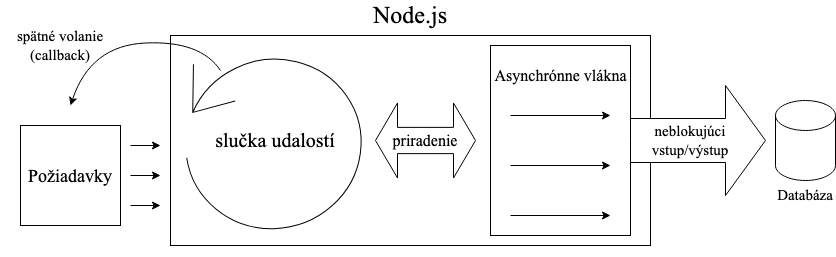
\includegraphics[scale=0.5]{obrazky/nodejs.png}
        \caption{Architektúra Node.js.}
        \label{pic:nodejs}
    \end{figure}
    
\subsection*{Express.js}
\label{express}
Express.js\cite{expressjs} je najpopulárnejším webovým frameworkom založeným na Node.js. Je minimalistický a flexibilný. Poskytuje robustnú škálu funkcionalít pre tvorbu serverovej časti webových aplikácií a množstvo HTTP utilít pre rýchlu a jednoduchú tvorbu aplikačného rozhrania. Umožňuje spracovanie jednotlivých HTTP dotazov na rôzne URL adresy.

\subsection{Aplikačné rozhranie}
\label{api}
Aplikačné rozhranie je realizované pomocou architektúry REST. Skratka znamená Representation State Transfer, čiže reprezentačný prenos stavu. Architektúra umožňuje pristupovať k dátam a vykonávať nad nimi základné operácie, ako ich vytvorenie, čítanie, aktualizáciu a mazanie. Na prenos dát sa používajú metódy protokolu HTTP. Najčastejšie používané metódy sú:

    \begin{itemize}
        \item\texttt{GET} pre získanie dát.
        \item\texttt{POST} pre vytváranie dát.
        \item\texttt{DELETE} pre mazanie dát.
        \item\texttt{PUT} pre upravovanie dát.
    \end{itemize}
    
Protokol ponúka aj metódy \texttt{HEAD}, \texttt{PATCH}, \texttt{OPTIONS}, ktoré avšak nie sú často používané.

\vspace{\baselineskip}

Architektúra poskytuje pre každý jeden zdroj samostatný koncový bod cez ktorý sa dajú dáta spravovať. Tabuľka koncových bodov použitých v aplikácii s ich popisom sa nachádza v sekcii \ref{table:endpoints}.

Aplikačné rozhranie musí splňovať nasledujúce požiadavky, aby bola považovaná za RESTful:

    \begin{itemize}
        \item\textbf{Klient-server architektúra} - cieľom je rozdeliť klientskú časť aplikácie od serverovej. Umožňuje nezávislý vývoj oboch častí aplikácie. Užívateľské rozhranie na viacerých platformách môže mať rovnaký backend.
        \item\textbf{Bezstavová architektúra} - požiadavky na server musia obsahovať všetky potrebné informácie na ich spracovanie. Stav sa uchováva na strane klienta a nie na strane servera.
        \item\textbf{Uchovávateľnosť v cache pamäti} - kvôli vysokému počtu požiadavkov, každý jeden požiadavok musí byť označený ako uložiteľný, alebo neuložiteľný do cashe pamäte. Výsledkom je zefektívnená výkonnosť servera.
        \item\textbf{Vrstovateľnosť} - rozdelenie aplikácie do jednotlivých vrstiev, kvôli škálovateľnosti. Každá vrstva má svoj vlastný účel.
        \item\textbf{Jednotné rozhranie} - základ architektúry, musí byť zadefinovaný spôsob komunikácie medzi klientom a serverom.
        \item\textbf{Code on Demand} - voliteľný požiadavok architektúry. Umožňuje posielanie zdrojového kódu pre klienta, čím rozšíri jeho funkcionalitu.
    \end{itemize}

\subsection{Ostatné balíčky a knižnice}
\subsection*{bcrypt}
Bcrypt je knižnica pre Node.js, ktorá umožňuje hašovanie hesiel.

\subsection*{cors}
Knižnica poskytuje middleware pre Express.js, ktorý povoluje zdieľanie zdrojov medzi inými doménami(cross-origin resource sharing).

\subsection*{day.js}
Day.js je minimalistická JavaScript knižnica pre prácu s časom a dátumom.

\subsection*{dotenv}
Modul načíta premenné zo súboru prostredia \texttt{.env} a prístupní ich cez objekt \texttt{process.env}.

\subsection*{jsonwebtoken}
Knižnica implementuje autentifikáciu užívateľa cez JSON Web Token. Implementácia autentifikácie pomocou tejto knižnice je podrobnejšie popísana v sekcii \ref{jwtauth}.

\subsection*{ts-node, tslint a typescript}
Knižnice ts-node a typescript slúžia pre spustenie prostredia Node.js s podporou pre jazyk TypeScript. Knižnica tslint je nástroj pre analýzu zdrojového kódu v jazyku TypeScript.

\subsection*{nodemon}
Nodemon je nástroj pre vytvorenie vývojového prostredia Node.js aplikácie, ktorý automaticky aktualizuje aplikáciu pri detekovaní zmeny v zdrojových súboroch. Vývojové prostredie sa vytvorí pomocou príkazu v terminály:
\begin{verbatim}nodemon ts-node ./src/server.ts
\end{verbatim}
